%----------------------------------------------------------------------------------------
%	PACKAGES AND OTHER DOCUMENT CONFIGURATIONS
%----------------------------------------------------------------------------------------

\documentclass{article}
\usepackage{mathtools}
\usepackage{float}

%----------------------------------------------------------------------------------------
%	PACKAGES AND OTHER DOCUMENT CONFIGURATIONS
%----------------------------------------------------------------------------------------

\usepackage{amsmath,amsfonts,stmaryrd,amssymb} % Math packages

\usepackage{enumerate} % Custom item numbers for enumerations

\usepackage[ruled]{algorithm2e} % Algorithms

\usepackage[framemethod=tikz]{mdframed} % Allows defining custom boxed/framed environments

\usepackage{listings} % File listings, with syntax highlighting
\lstset{
	basicstyle=\ttfamily, % Typeset listings in monospace font
}

%----------------------------------------------------------------------------------------
%	DOCUMENT MARGINS
%----------------------------------------------------------------------------------------

\usepackage{geometry} % Required for adjusting page dimensions and margins

\geometry{
	paper=a4paper, % Paper size, change to letterpaper for US letter size
	top=2.5cm, % Top margin
	bottom=3cm, % Bottom margin
	left=2.5cm, % Left margin
	right=2.5cm, % Right margin
	headheight=14pt, % Header height
	footskip=1.5cm, % Space from the bottom margin to the baseline of the footer
	headsep=1.2cm, % Space from the top margin to the baseline of the header
	%showframe, % Uncomment to show how the type block is set on the page
}

%----------------------------------------------------------------------------------------
%	FONTS
%----------------------------------------------------------------------------------------

\usepackage[utf8]{inputenc} % Required for inputting international characters
\usepackage[T1]{fontenc} % Output font encoding for international characters

\usepackage{newtxtext} % Use the XCharter fonts

%----------------------------------------------------------------------------------------
%	COMMAND LINE ENVIRONMENT
%----------------------------------------------------------------------------------------

% Usage:
% \begin{commandline}
%	\begin{verbatim}
%		$ ls
%		
%		Applications	Desktop	...
%	\end{verbatim}
% \end{commandline}

\mdfdefinestyle{commandline}{
	leftmargin=10pt,
	rightmargin=10pt,
	innerleftmargin=15pt,
	middlelinecolor=black!50!white,
	middlelinewidth=2pt,
	frametitlerule=false,
	backgroundcolor=black!5!white,
	frametitle={Command Line},
	frametitlefont={\normalfont\sffamily\color{white}\hspace{-1em}},
	frametitlebackgroundcolor=black!50!white,
	nobreak,
}

% Define a custom environment for command-line snapshots
\newenvironment{commandline}{
	\medskip
	\begin{mdframed}[style=commandline]
}{
	\end{mdframed}
	\medskip
}

%----------------------------------------------------------------------------------------
%	FILE CONTENTS ENVIRONMENT
%----------------------------------------------------------------------------------------

% Usage:
% \begin{file}[optional filename, defaults to "File"]
%	File contents, for example, with a listings environment
% \end{file}

\mdfdefinestyle{file}{
	innertopmargin=1.6\baselineskip,
	innerbottommargin=0.8\baselineskip,
	topline=false, bottomline=false,
	leftline=false, rightline=false,
	leftmargin=2cm,
	rightmargin=2cm,
	singleextra={%
		\draw[fill=black!10!white](P)++(0,-1.2em)rectangle(P-|O);
		\node[anchor=north west]
		at(P-|O){\ttfamily\mdfilename};
		%
		\def\l{3em}
		\draw(O-|P)++(-\l,0)--++(\l,\l)--(P)--(P-|O)--(O)--cycle;
		\draw(O-|P)++(-\l,0)--++(0,\l)--++(\l,0);
	},
	nobreak,
}

% Define a custom environment for file contents
\newenvironment{file}[1][File]{ % Set the default filename to "File"
	\medskip
	\newcommand{\mdfilename}{#1}
	\begin{mdframed}[style=file]
}{
	\end{mdframed}
	\medskip
}

%----------------------------------------------------------------------------------------
%	NUMBERED QUESTIONS ENVIRONMENT
%----------------------------------------------------------------------------------------

% Usage:
% \begin{question}[optional title]
%	Question contents
% \end{question}

\mdfdefinestyle{question}{
	innertopmargin=1.2\baselineskip,
	innerbottommargin=0.8\baselineskip,
	roundcorner=5pt,
	nobreak,
	singleextra={%
		\draw(P-|O)node[xshift=1em,anchor=west,fill=white,draw,rounded corners=5pt]{%
		Question \theQuestion\questionTitle};
	},
}

\newcounter{Question} % Stores the current question number that gets iterated with each new question

% Define a custom environment for numbered questions
\newenvironment{question}[1][\unskip]{
	\bigskip
	\stepcounter{Question}
	\newcommand{\questionTitle}{~#1}
	\begin{mdframed}[style=question]
}{
	\end{mdframed}
	\medskip
}

%----------------------------------------------------------------------------------------
%	WARNING TEXT ENVIRONMENT
%----------------------------------------------------------------------------------------

% Usage:
% \begin{warn}[optional title, defaults to "Warning:"]
%	Contents
% \end{warn}

\mdfdefinestyle{warning}{
	topline=false, bottomline=false,
	leftline=false, rightline=false,
	nobreak,
	singleextra={%
		\draw(P-|O)++(-0.5em,0)node(tmp1){};
		\draw(P-|O)++(0.5em,0)node(tmp2){};
		\fill[black,rotate around={45:(P-|O)}](tmp1)rectangle(tmp2);
		\node at(P-|O){\color{white}\scriptsize\bf !};
		\draw[very thick](P-|O)++(0,-1em)--(O);%--(O-|P);
	}
}

% Define a custom environment for warning text
\newenvironment{warn}[1][Warning:]{ % Set the default warning to "Warning:"
	\medskip
	\begin{mdframed}[style=warning]
		\noindent{\textbf{#1}}
}{
	\end{mdframed}
}

%----------------------------------------------------------------------------------------
%	INFORMATION ENVIRONMENT
%----------------------------------------------------------------------------------------

% Usage:
% \begin{info}[optional title, defaults to "Info:"]
% 	contents
% 	\end{info}

\mdfdefinestyle{info}{%
	topline=false, bottomline=false,
	leftline=false, rightline=false,
	nobreak,
	singleextra={%
		\fill[black](P-|O)circle[radius=0.4em];
		\node at(P-|O){\color{white}\scriptsize\bf i};
		\draw[very thick](P-|O)++(0,-0.8em)--(O);%--(O-|P);
	}
}

% Define a custom environment for information
\newenvironment{info}[1][Info:]{ % Set the default title to "Info:"
	\medskip
	\begin{mdframed}[style=info]
		\noindent{\textbf{#1}}
}{
	\end{mdframed}
}
 % Include the file specifying the document structure and custom commands

%----------------------------------------------------------------------------------------
%	ASSIGNMENT INFORMATION
%----------------------------------------------------------------------------------------

\title{Cryptography, ITC8240 Assignment \#3} % Title of the assignment

\author{Oskar Pihlak} % Author name and email address

\date{TalTech --- \today} % University, school and/or department name(s) and a date

%----------------------------------------------------------------------------------------

\begin{document}

\maketitle % Print the title

%----------------------------------------------------------------------------------------
%	INTRODUCTION
%----------------------------------------------------------------------------------------

\section*{Introduction} % Unnumbered section

This is the Assignment \#3 submission for the Cryptography course, written in LaTeX.\\



%----------------------------------------------------------------------------------------
%	2.1 TASK 1
%----------------------------------------------------------------------------------------

\section*{Task 1 (12 points) - Groups and Number theory} % Numbered section
\begin{itemize}
    \item Is ($Q$, $+$) (Rationals under addition) a group? Motivate your answer.
\end{itemize}
asdasdasdasd

\begin{itemize}
    \item Is ($Z_{33}$ \textbackslash {0}, \text{*}) (Integers modulo $33$ excluding $0$ under multiplication ) a group ? Motivate your answer.
\end{itemize}
asdasd

\begin{itemize}
    \item Write down a definition of homomorphism. Show a homomorphism
    between ($Z, +$) and ($R^+$, \text{*}).
\end{itemize}
asdasdasd

\begin{itemize}
    \item Estonian boatswain is trying to sell corsair Alice a sailboat, however without revealing the age of the sailboat. 
    From several sailors Alice found that one year ago, its age was a multiple of $4$, in $3$ years its age will be a multiple of $7$, 
    and in $5$ years multiple of $11$. Help Alice to deduce the age of the sailboat. Do not skip calculations in this solution!!!.
\end{itemize}
asdasdasd

\begin{itemize}
    \item Calculate the order of $7$ in ($U^{\text{*}}_{15}, \text{*}$) (set of units).
\end{itemize}
asdasdasd

\begin{itemize}
    \item Calculate Euler’s totient function for number $55440$.
\end{itemize}
asdasdasd


\begin{itemize}
    \item Calculate and provide intermediate calculations $$(-14)^{42}~mod~1181$$ 
\end{itemize}
asdasdasd



\section*{Task 2 (7 points) - Probability theory} % Numbered section
\begin{itemize}
    \item The box contains $3$ white balls and $2$ black ones. One ball is drawn from the box, and then the second. Event $B$ - the 
    appearance of a white ball at the first draw. Event $A$ - the appearance of a white ball on the second draw. Find $P(A|B)$ and $P(A|\overline{B})$
\end{itemize}
asdasdasd

\begin{itemize}
    \item Among the $30$ cryptography exam variants, there are $7$ ”lucky”. Two students take turns taking one variant 
    (the first student takes each of the variant with the same probability, the second - equally likely any of the remaining ones). 
    Find the probability that the second student took the ”lucky” variant. Write your answer as a fraction $\frac{X}{Y}$.
\end{itemize}
asdasdasd

\begin{itemize}
    \item Cryptography students is solving multiple choice task. There are n options. 
    If cryptography student knows a solution, they choose the right option. 
    If they do not - they randomly choose the answer with probability $\frac{1}{n}$. 
    What is the probability, that student knows a solution for a task, under a condition that they chose the right option? 
    (Hint: a) treat probability of student knowing the answer as parameter b) Bayes formula.
\end{itemize}
asdasdasd

\section*{Task 3 (8 points) - RSA} % Numbered section
\begin{itemize}
    \item Show that RSA is not ND-CCA2. The IND–CPA game is defined as follows.
\end{itemize}
\begin{figure}[H]
    \centering
    \label{fig:task3pic0}
    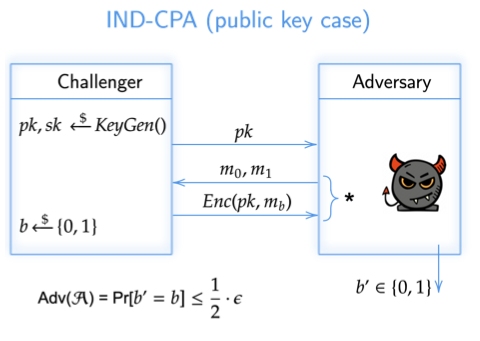
\includegraphics[scale=0.5, angle=0]{task3_pic0.png}
    \caption{Auction setup.}
\end{figure}

asdasd

\begin{itemize}
    \item Imagine the following modification to the $RSA$ encryption scheme. 
    Instead of generating $p$ and $q$ as a distinct prime numbers, we set $q = p$
    (i.e. modulus $n = p^2$). All other steps remain the same. Please, explain, 
    is the security of the scheme affected by this change? If yes, please provide an attack.
\end{itemize}

asd

\section*{Task 4 (6 points) - ElGamal encryption} % Numbered section
\begin{enumerate}
    \item Consider the ElGamal cryptosystems with a public key $(p,q,y)$ and a private key $x$. Encrypt the message $m = 15131$ 
    using parameters $p = 199999$,~$q = 23793$,~$x = 894$,~$r = 723$. Decrypt the ciphertext $c = (299,457)$ using parameters $p = 503$, $q = 2$, $x = 42$.
\end{enumerate}

\begin{enumerate}
    \setcounter{enumi}{1}
    \item Assume there is an jewellery auction happening, both Alice and Eve want to buy precious diamond earrings. 
    The rules of the auction are the following:
    \begin{itemize}
        \item Each bidder places a bid.
        \item The highest bidder gets the first slot, the second-highest, the second slot and so on.
        \item The highest bidder pays the price bid by the second-highest bidder.
    \end{itemize}
\end{enumerate}
\begin{figure}[H]
    \centering
    \label{fig:task4pic0}
    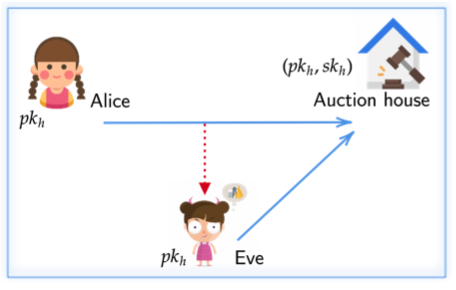
\includegraphics[scale=0.5, angle=0]{task4_pic0.png}
    \caption{Auction setup.}
\end{figure}

Eve found out that the bids are sent to the auction house in encrypted form, using ElGamal encryption. Additionally, 
Eve can eavesdrop on communication between Alice and auction house. Explain, how can Eve win the auction using homomorphic properties of ElGamal.

\section*{Task 5 (9 points) - Hash functions and signatures} % Numbered section
\textbf{Part 1.} Let p be a prime number and let $g$ be a generator of $Z^{\text{∗}}_{p}$. Suppose we have the following 
function: $f : Z \rightarrow Z^{\text{*}}_{p}$, where $f(x) = g^{x}~mod~p$. Is $f$ collision resistant? Please, explain your answer.
\\ \\
asd
\\ \\
\textbf{Part 2.} Assume Alice uses some signature algorithm $S$ with a hash function $H$ that is not collision resistant. 
That is, to sign a message $m$ Alice first computes $H(m)$ and then uses some secret key to sign $H(m)$. 
Explain, how malicious Carl can trick Alice into signing a fraudulent document.
\\ \\ 
asd


\end{document}
